The review and synthesis of existing literature is foundational for new research and critical to the dissemination of results to other researchers and to external communities (i.e. industrial practitioners). 
A literature review can have various goals, e.g., grounding new work in previous findings or synthesizing the current state of knowledge.
Unfortunately, literature reviews in SE are still too often performed in an \textit{ad hoc} manner -- thus producing results that may be biased, less than comprehensive, not repeatable, or inconclusive.

To provide structure to the literature review process, medical researchers defined the SLR approach. 
Figure~\ref{figure-SLR-Process} provides an overview of the SLR process, which is described in more detail in Section~\ref{sec:process}.
An SLR is a formal, repeatable approach by which a team of researchers can identify, evaluate, synthesize, and interpret the available research about a question or topic area. 
In an SLR, the researchers develop and validate a detailed plan for searching the literature, identifying and selecting studies, extracting data, and finally analyzing and synthesizing that data.

\begin{figure}
	\centering
	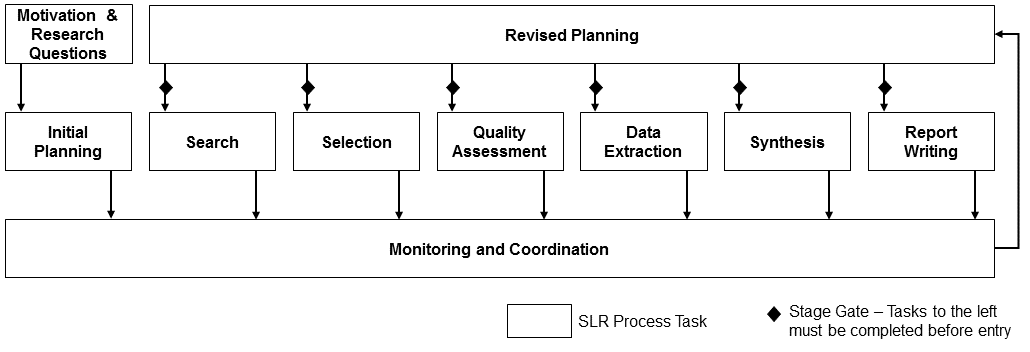
\includegraphics[width=\textwidth]{SLR_Process_Flow}
	\caption{SLR Process Flow}
	\label{figure-SLR-Process}
\end{figure}

Medical researchers, practitioners, and policy makers have long relied on SLRs because they integrate up-to-date, reliable, and critical information that supports important decisions.
Seeking these same benefits, in the last decade, SE researchers have embraced Evidence-Based Software Engineering~\cite{Kitchenham-etal:04, Kitchenham:04} and specifically SLRs.
Indeed, with the growing emphasis on empirical research in SE, SLRs are of critical importance because they allow researchers to gather disparate evidence to understand the effects various SE tools, techniques and methods have on industrial practice. 
SE researchers have published more than 300 SLRs on a wide range of topics.

Even with this success, the question arises: \textit{How can we ease the burden on SE researchers who conduct SLRs and encourage SE researchers to conduct more SLRs?} 
Results from our previous work (i.e. 2 international workshops, a review of over 200 published SLRs, and a survey of over 50 SLR authors) and our own experiences have converged to indicate that the primary barriers to conducting SLRs are the fact that they are difficult, time-consuming, and lack an integrated tool set.  
Based on our previous work, we have identified four guiding principles for the development of a successful SLR support infrastructure to overcome these barriers.

\textbf{Principle 1: Automate the SLR process to reduce manual labor and allow for iteration.}
Portions of the SLR process are ripe for automation, with the appropriate infrastructure.
For example, SE researchers lack adequate tools to assist in the searching and identification of relevant published research.
The presence of multiple SE literature databases (e.g., IEEExplore, ACM, or Google Scholar), each of which have different search functionality and interfaces, necessitates a federated approach that can search all databases simultaneously and de-duplicate the results. 
In addition, automation of the SLR process will allow researchers to more easily iterate among phases.

\textbf{Principle 2: Facilitate collaboration.}
The SLR process by its very nature is collaborative.
To reduce the effects of single-researcher bias, multiple researchers must collaboratively execute the SLR process by reviewing and synthesizing research from the published literature.
Our review of published SLRs indicates that the average number of authors is three.
There are currently few tools to effectively support this collaboration throughout the SLR process.
Therefore, there is a need to enable collaboration both among co-located teams (e.g. PhD students and their advisor) and among distributed teams (e.g. researchers from different countries).

\textbf{Principle 3: Store data to support reuse and evolution.}
It is likely that the same paper may be relevant to multiple SLRs. 
Because there is no central repository for storage of extracted data, researchers must fully repeat this extraction process for each new SLR. 
Providing persistent data storage of extracted information would both reduce effort, by enabling a researcher to extract only the additional data relevant to the new research question(s), and facilitate collaboration, by allowing researchers to identify others working on similar topics.
In addition, storage of data in a central repository will facilitate the goal of making SLRs into ``living'' documents that can evolve as new research is published.
Researchers can more easily integrate new findings with the existing results by taking advantage of the access to stored data.

\textbf{Principle 4: Provide an open ecosystem to enable the use of external tools.}
There are a number of existing tools, and groups working on new tools, that support some aspects of the SLR process (see Section~\ref{sub:existing:tools}).
By allowing tool authors to integrate their tools into our environment and by providing access to the persistent data store, we will increase the overall value of this infrastructure.

Driven by these key principles, the goal of this CI-NEW grant is to \textbf{build upon our CI-P results to implement the SLR Authoring Infrastructure Toolkit (SAInT) that will be beneficial to SE by removing barriers to the conduct of SLRs and encouraging more widespread adoption of the SLR approach.}

Once deployed, SAInT will reduce the resource impedance SE researchers face in the rigorous, labor-intensive process required to conduct literature reviews that are systematic, comprehensive, and reproducible.  
\textit{As can be seen in other disciplines such as medicine, identifying, evaluating, and synthesizing the existing body of literature is time consuming but is critical to both extend research and improve practice outcomes.}
SE researchers will benefit from SAInT because its tools will enable free-standing, independent reviews that summarize and integrate existing evidence, identify gaps in current research and provide a framework for positioning new research. 
Moreover SAInT will provide a common interchange of SLR metadata among toolsmiths and support the community around which a SE SLR ecosystem can advance.

The proposal is organized as follows. 
Section~\ref{sec:process} provides background on SLRs.
\ref{sec:identification:needs} motivates the need for the proposed infrastructure including identification of the CISE constituent community (Section~\ref{sec:community:needs}) and the results of our planning grant (Section~\ref{sec:planning:results}).
\ref{sec:research:enabled} describes the research enabled by the proposed infrastructure. 
\ref{sec:implementation} details the implementation and evaluation plan for the proposed infrastructure. 
\ref{sec:plan} lays out the project plan. 
Finally,~\ref{sec:IMBI} describes the Intellectual Merits and Broader Impacts of the proposed work.
